\chapter{Methods}
\label{ch:methods}

\section{Methodology}

My methodological approach is cross-disciplinary and exploratory.
%
The cross-disciplinary aspect is inherent in the topic; it would
be impossible to characterise Indigenous seasons in this way without
integrating qualitative and quantitative methods.
%
It is exploratory because there is no known precedent or published
method for quantification of an Australian Indigenous seasonal calendar.
This novelty means that the specific quantification methods used
were not known ahead of time, as they are informed and shaped by
interview data.  It also means that these methods themselves form
a novel result, which breaks ground for further research.

My specific methods fall into four distinct stages.
\begin{enumerate}
\item Draw on literature describing the Yolngu seasonal calendar
\item Interviews with Yolngu and non-Indigenous people who
    understand this calendar
\item Quantitative methods bridging literature and interview
    descriptions to the observational weather record, to characterise
    Yolngu seasons
\item Analysis of the derived seasonal record, such as typical
    conditions for each season and correlations with climate indicies.
\end{enumerate}
These stages reflect the cross-disciplinary or mixed-methods approach --
literature informing the direction of the research, and qualitative
methods providing the framework for well-founded numerical analysis.


\paragraph{Qualitative research methodology} is particularly important
when working across cultures, for example when collaborating with
Indigenous people on western-style scientific research.
%
``Research'' is something of a dirty word in many Indigenous communities;
even where the people involved are trusted.  The most common experience
is one of exploitation or at least unequal benefits, where researchers
come and go, but leave nothing for the Indigneous participants.

Without strong pre-existing relationships, in my case through several
years of national work in the Uniting Church, this research would not
have been possible.  The trust earned through ongoing engagement allowed
me to commit to share my results and ensure that Yolngu participants will
also benefit from this study.  Without the introductions and logistical
assistance generously provided by the church, it would be impractical or
impossible to conduct such research for an Honours thesis.
%
In a letter inviting collaboration on this research (see \cref{sec:ethics}),
a senior Yonlgu man explained that
\begin{quote}
    For Yolngu (the people of North Eastern Arnhem Land) it is the Liyagadhaman
    who carry within them the wisdom and knowledge of these matters.
    It is right that in this research you have approached me to talk about these
    things. I can also introduce you to others who have this knowledge.
    ...
    Yolngu have made careful observation of the ways of nature and the seasons
    over the millennia and have passed on that knowledge down the generations.
    We know the changes that are taking place in the seasons and I am willing
    to talk with you about what I have seen happening around me.
\end{quote}


\paragraph{Data scoping} is a key influence on methodology.
What data is within scope or relvant to the research question --
and what isn't?
%
This question is decided by a combination of principles and pragmatism;
the data must be sufficient for robust and well-founded analysis,
and it must also be possible to aquire and understand with limited
resources.  Secondary considerations include the potential applications
of the results, and avoiding undue difficulty for replication.

On these grounds, both qualitative and numerical data focus on the present.
Interviews do not attempt to investigate historical understandings of
seasons or calendars, and are conducted in English -- linguistic or
anthropological study is firmly out of scope.

All numerical weather data are drawn from daily direct observations at
surface weather stations.  Other datasets -- such as satellite observations,
climate models, etc -- generally do not have both the spatial and the
temporal resolution required, or are missing key variables such as seperate
surface wind vectors for morning and afternoon.
%
The Australian Bureau of Meteorology generously provided the data for each
weather station in the study area (included in the electronic appendices).
Similar data -- with the notable exception of wind -- is freely available
for many other stations, which may encourage replication for other
calendars.


\paragraph{Context}

This study will explore Yolngu seasons, using the towns of Galiwinku and
Milingimbi as a case study for practical reasons.  Personal connections and
logistical support from the Uniting Church facilitate fieldwork with limited
resources.  Yolngu seasons emphasise meteorological indicators, which allow
principled quantification based on the observational weather record.
%
The study area is on the north-east coast of the Northern Territory, shown
in  \cref{fig:arnhem-map}, about five hundred kilometers east of Darwin.
These sites fall within the Anrhem Coast bioregion \citep{ens2014}.
The landscape is dominated by tropical woodland, from mangroves on the
coastline through dense forest to more open woody grasslands further inland.
Qualitative seasonality is described for Galiwinku and Milingimbi;
quantitative weather observations from Waruwi, Maningrida, Milingimbi,
will also be analysed.  Waruwi and Maningrida are in areas described by
other calendars, but provide a longer weather record in a similar climate.

\begin{figure}[h]
    \centering
    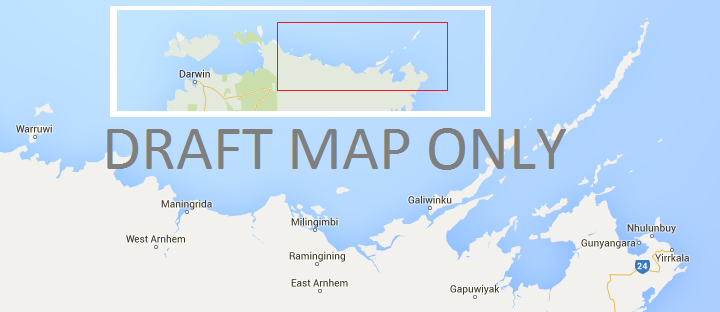
\includegraphics[width=\textwidth]{mapdraft.png}
    \caption[Map showing the study area, NE Arnhem Land]{
        Map showing the study area, NE Arnhem Land.
        Analysis in \cref{ch:quantify} uses weather observations from several of the towns shown.
        \todo{better map (inset all Aus), label towns and referenced place names
        (Elcho Island, etc.)
        Would also be good to shade by Indigenous group, approximately.}
        }
    \label{fig:arnhem-map}
\end{figure}



\paragraph{Season recognition} is difficult to encode, and my methods can
best be described as exploratory.  The specifics are described in
\cref{sec:applying-seasons-method}, as they closely follow qualitative
findings and constitute a result in themselves.

The general approach is to observe that seasons are recognised or defined
at least partially by weather conditions on a day-to-day basis.  It is
therefore possible to construct criteria for each season that describe
it in terms of daily weather observations, and derive an daily index for
each season.  Normalising these indicies by z-score makes them directly
comparable, and the season with the greatest index on some day is said
to occur on that day.

Alternative approaches, such as definitions by trend change in weather
or onset thresholds, are not supported by the qualitative data.  See
\cref{ch:results} for details.


\paragraph{Quantitative} summaries are an important aspect of this
research, but on the outer edge of it's scope.  This analysis is therefore
limited, to the extent that it either informs judgement of earlier work
or demonstrates potential for further study in a particular area.
%
In practice, this means calculating a small number of summary statistics
-- those which are meaningful for a complex calendar and supported by the
data -- and proof-of-concept analysis of Yolngu seasons with respect to
a few climate indicies.



\section{Qualitative and Interview Methods}

This research was approved by the ANU Human Research Ethics Committee.
Details of the approval can be found in \cref{sec:ethics}.
I rely on three sources of qualitative knowledge and context for the Yolngu
seasons.  Interviews with Yolngu people form the basis of my qualitative
research, and are the definitive source of information about Yolngu seasons.
Interviews and discussion with non-Indigenous researchers or teachers with
experience in remote communities contextualises this knowledge, and warned of
common misinterpretations - as well as pointing out nuance.

The two primary sources are contextualised and supported by published
literature on cross-cultural research \citep[eg.][]{smith1999}, Australian
Indigenous seasons \citep[eg.][]{prober2011,oconnor2010}, and Yolngu seasons
\citep{davis1989,atlas2014}.  Secondary sources shape the specific methods
and interview questions (below), or in the case of grey literature --
posters produced for remote schools, workbooks for cross-cultural teacher
training, etc. -- provided a starting point for informal conversations.


Prior to fieldwork, the planned sample was ten to twenty Yolngu people
of varied age and gender; interviews were to be conducted at Galiwinku
on Elcho Island, with supplementary interviews in Darwin.  Unfortunately
Rronang Garrawurra, who had offered his assistance with introductions
and accomodation (see \cref{app:invitation-letter}), was in Darwin due
to health issues and alternative accomodation was unavailable.

Fieldwork and interviews were ultimately conducted in Darwin.  Sample
recruitment followed a `snowball' pattern, where participants were asked
to suggest further potential participants \citep{patrick1996}.  The `seeds'
of this pattern were personal contacts in the Uniting Church, and the
CSIRO Tropical Rivers and Coastal Knowledge team \citep{CSIROcals}.

The final interview sample consisted of three older Yolngu men, four past
or practising teachers with several years experience in Arnhem Land, and
the CSIRO team.  Most participants asked not to be identified, so comments
are not attributed to individuals.


I conducted a series of informal, semistructured interviews discussing
seasons and climate.  Thematic questions include:
\begin{itemize}
\item What are the names of the seasons?
\item When does [a season] usually occur?  How do you know when it starts (definition)?
\item How long does [a season] last?  What weather or events usually occur in this season?
\item Do you think the seasons have changed over your lifetime?  Why/why not?  How can you tell?
\item Are there some years where a season is skipped?  What happens?
\item Do you remember any unusual events?  What happened?
\item What might the calendar be like if [example climate impact] happened?
      (eg changes to wind, temperature, rainfall patterns)
\end{itemize}

Interviews generally took the form of participant-led discussion prompted
by one of the thematic questions; the most consistently productive were
focussed on teaching about seasons: names and definitions, typical conditions
and timing, and touching on extreme events and outliers.
%
These discussions took place in venues suggested by the participant, often
under a tree by the ocean, at a cafe, or in their home.  Each discussion
lasted between one and two hours; I met with some participants multiple times
to discuss various aspects of Yolngu seasonality.

Just as Yolngu people offered their knowledge of seasons, discussions with
non-Indigenous people provided context and interpretative assistance as well
as their perspective on Yolngu seasons.  Immediate clarification and
feedback allowed for ongoing refinement of the questions, and suggested
new directions or overlooked details which were elicited in subsequent
interviews.

Following the interviews, I also engaged in substantial reflection on the nature
of my questions and the ambiguity of the responses and data I collected.
In this process, allowing participants to discuss whatever they felt relevant
is a key way to remain open to unexpected information - including insights
which changed my understanding of what a Yolngu seasonal calendar was!



\section{Application: from Qualitative to Numerical Data}

This paper attempts to quantify only one Yolngu seasonal, with six seasons
each year defined by weather conditions and events.  See
\cref{subsec:three-seasons-scales} for a brief explanation of other
Yolngu seasonal calendars, and an explanation of this focus.

\subsection{Weather Observations}

The key meteorological aspects of Arnhem Land seasonality are temperature,
rainfall, humidity, and wind strength and direction; the annual
cycle is driven primarily by the Indian Ocean monsoon.  The climate is hot and
humid, with daytime temperatures between 25 and 40 degrees year-round.
%
The numerical weather data were generously supplied by the Australian
Bureau of Meterology.  This section describes the basic numerical data,
quality checks, and handling of missing data.
The record begins with the installation of automatic weather stations
at several airports between 1990 and 2003  (some earlier observations exist,
but do not include all required variables).  The results do not support
speculatation on the past or future state of Yolngu seasons.  The methods
however are applicable to data such as climate models, which provide
a clear direction for further work.

\begin{table}[h]
    \caption[List of weather stations providing data]{
        Summary description of weather stations used.
        Locations are visible in \cref{fig:arnhem-map}}
    \label{tab:weather-station-summary}
    \sffamily\small
    \centerline{
    \begin{tabular}{cllcccl}
        Station no.  &  Name                &  Location    &  Latitude  &  Longitude   &  Altitude  &  Opened   \\
        \noalign{\vskip 0.5em}\hline\noalign{\vskip 0.5em}
        014401       &  Warruwi Airport     &  Warruwi     &  11.6500S  &  133.3797E   &  19m       &  Jan 1916 \\
        014404       &  Milingimbi Airport  &  Milingimbi  &  12.0932S  &  134.8919E   &  15m       &  Mar 2003 \\
        014405       &  Maningrida Airport  &  Maningrida  &  12.0569S  &  134.2339E   &  28m       &  Oct 2003 \\
        014508       &  Gove Airport        &  Nhulunbuy   &  12.2741S  &  136.8203E   &  52m       &  Jan 1944 \\
        014517       &  Ngayawili           &  Galiwinku   &  11.9971S  &  135.5726E   &  08m       &  Oct 1999
    \end{tabular}
    }
\end{table}

\Cref{tab:weather-station-summary} shows the name, ID, and location of
the weather stations used.
%
The weather variables of interest are:
\begin{itemize}
\item Rainfall in the 24 hours before 9am (local time), in milimeters.
\item Maximum temperature in the 24 hours after 9am (local time), in Degrees C.
\item Minimum temperature in the 24 hours before 9am (local time), in Degrees C.
\item Humidity measured as average daily dew point temperature, in Degrees C.
\item Wind speed measured in kilometers per hour, at 9am and 3pm local time.
\item Wind direction recorded as 16 compass points, at 9am and 3pm local time.
\end{itemize}

Participants suggested that season detection should not consider 3pm wind
due to the effect of the sea breeze, and that 6pm would be more suitable.
\Cref{fig:galiwinku-seabreeze-direction} shows wind direction by year
and day-of-year, as in \cref{fig:galiwinku-observations}.
%
Similar charts for wind speed and other stations are included in the electronic
appendices.  These charts show a northerly sea breeze, generally strong in the
noon, 3pm, and 6pm data.  I use 3pm wind data, as these comments are outweighed
by the standard time and longer record at some stations.

The data are cleaned by discarding observations accumulated over multiple days.
Observations which have been quality-controlled by the BoM and are considered
`wrong', `suspect', or `inconsistent with other known information' are discarded.
Observations which have not been assessed are retained.
%
Missing data is not filled in any way, to convey the coverage of the record
and accurately represent missing data in the figures.  In scalar calculations,
missing data is propagated (eg ${NaN+10=NaN}$); in some aggregation
it is omitted from the sample (eg ${mean(1,NaN,5)=3}$, though
${mean(NaN,NaN)=NaN}$). Heatmap figures represent missing data as a black cell.


\subsection{Detection of Seasons}

Seasons are detected at daily resolution, matching the input weather data.
Each of these methods assigns a confidence rating for each season to each day of
observations.  These ratings are then reconciled to a single season, or unknown,
for each day.  The reconciliation draws on participants' comments to drop inconsistent
ratings before comparing normalised season ratings.

For each season, I construct a set of boolean criteria based on participant
descriptions.  A raw index for each season is defined by
running these conditions over each day of data (giving True, False, or NaN),
and summing the values for each season for each day (giving NaN, 0, 1, ...).
\Cref{fig:season-definitions-code} shows the code used to build raw
seasonal indicies.

Season-detection criteria can be defined in two ways: based on thresholds
in absolute measurement, or on trends.  I prefer the threshold approach,
as experimenting with trend-based detection did not yield reliable results.
While I consider changes in the weather a better fit for season detection,
and a strong area for further study, this approach is impractical given available
qualitative and quantitative data.

These thresholds are set based on the calendar described in \cref{sec:calendar-description};
for categorical criteria such as wind direction or the absence of rain days
I am confident that they are reasonably rigorous.  For quantitative criteria,
such as ``very hot'', ``humid'', rain on ``most days'' or ``less frequently'',
rigour is more dificult.

The ideal solution would be to find a historical record of what season
it was on various days; regression analysis, (un)supervised classification,
or machine learning techniques could then associate seasons with typical
conditions.  Unfortunately, no such record exists -- in searching for one
I spoke to Yolngu people, current and ex-mission workers, the Tropical
Rivers and Coastal Knowledge team at CSIRO, academics from Charles Darwin
University and Nungalinya College.

Instead, I tried a range of values and selected those which appeared to
best reproduce the described timing of each season in the Galiwinku and
Milingimbi data.  This selection was on the basis of normalised season
indicies before aggregation, so it tested for specific descriptions
rather than merely expected results.
%
This is probably the weakest step in the quantification method, but the data
required for more rigorous fitting of these parameters is not available.
Examination of figures for unfitted weather stations (see electronic appendices)
shows good agreement, suggesting that this method is sufficient for exploratory
analysis.

Finally, the index timeseries for each season is normalised by conversion to
a z-score, to allow direct comparison between seasons - the variation in data
completeness and number of conditions would not otherwise permit it.
This index is my representation of how well the season characterises that day's
conditions.  Aggregation of these indicies is covered in the next section.



\section{Quantitative Analysis}

All numeric tables and data visualisations in this thesis are produced
with Python scripts writen by the author.  The raw data supplied by the
Bureau of Meteorology are supplied in the electronic appendices, as
are the analysis scripts.  This makes all quantitative results trivial
to reproduce, and greatly facilitates replication for other calendars
or datasets.  Running the scripts requires Python version 3.5 or later,
as well as the Pandas (0.18+) and Seaborn (0.7+) libraries with their
dependencies.

Seasons may occur multiple times in a given year, in any order (see
\cref{subsec:detection-advice} for an explanation).  This presents a significant
challenge to reliable detection of seasonal onset, as it rules out
the simple approach of detecting an event and forward-filling the
associated season to the next detected event.  Instead, I use a local
analysis approach which seperately analyses each day of data with
a small window only used for smoothing via a rolling mean of 3-7 days.
%
The cost of this well-grounded system is increased `jitter', rapid
switching between seasons in periods when more than one is a close match
for conditions.  Future studies may wish to use an alogrithm that `remembers'
recent decisions, accounting for the advice that season change requires
several days observation.  This study prefers to avoid the risk of
over-fitting, sensitivity to initial conditions, and implementation
challenges such an approach brings.

In ny case, Yolngu seasons cannot be well characterised by onset timing.
Instead of asking ``when does [this season] typically begin?'' - which implies
that each season begins once per year, at a roughly constant date -
it is better to ask which season best matches conditions at a date,
or which is most commonly observed.
%
The benefits and drawbacks of various ways to characterise typical or onset
timing for seasons is discussed in \cref{subsec:disc-season-detection}.



~\\

Calculation of summary statistics for each season has a firmer conceptual
grounding.  The daily data are grouped by detected season and summary statistics
for each subset calculated, including measures of central tendency and
variation in ...
\begin{itemize}
\item Calculation of summary stats for each season � typical and variation in conditions, onset, etc
\item Comparison of stations, other data as inputs to season recognition.
\item Correlation to ENSO, monsoon, dipole moment, etc
\end{itemize}

Note that even the simplest of these is really novel, as nobody has
been able to calculate the summaries before!

